\section{溶液中各组分的化学势}


\begin{frame}
    \frametitle{纯物质液态的化学势}
    在每一个给定温度下，纯物质的液态都和自己在给定温度下的饱和蒸气处于热力学平衡。一般情况下，因为饱和蒸气的压强较低，所以它的化学势可以用理想气体的化学势代表。
    \begin{center}
        \begin{tikzpicture}[scale=1.5]
            \draw[fill=maincolor!30] (0,0) rectangle (3,1) node[midway] {液相};
            \draw[shift={(0,1)}] (0,0) rectangle (3,1) node[midway] {气相($p^*$)};
            \draw[->] (1.4,0.8)--(1.4,1.2);
            \draw[->] (1.6,1.2)--(1.6,0.8);
        \end{tikzpicture}
    \end{center}
    \[
        \mu_\mathrm{l}=\mu^*=\mu^\ominus(T) +R T \ln \frac{p^*}{p^{\ominus}}
    \]
\end{frame}


\begin{frame}{拉乌尔定律}
    拉乌尔(Raoult)根据大量的稀溶液实验发现，定温下{\color{red}稀溶液}的蒸汽压与溶液的组成具有线性关系。定温下，稀溶液中溶剂的蒸汽压$p_\mathrm{A}$等于该温度时纯溶剂的饱和蒸汽压$p_\mathrm{A}^*$与溶液中溶剂的摩尔分数$x_\mathrm{A}$的乘积。

    \begin{minipage}{0.58\linewidth}
        $$p_\mathrm{A}=p_\mathrm{A}^*x_\mathrm{A}$$
    若溶液仅由$x_\mathrm{A}$的A和$x_\mathrm{B}$的B两种组分构成，则$x_\mathrm{A}+x_\mathrm{B}=1$，拉乌尔定律可写成
    $$\frac{p_\mathrm{A}^*-p_\mathrm{A}}{p_\mathrm{A}^*}=x_\mathrm{B}$$
    溶液的蒸汽压降低与纯溶剂的饱和蒸汽压之比等于溶质的摩尔分数。
    \end{minipage}\hfill
    \begin{minipage}{0.38\linewidth}
        \begin{center}
            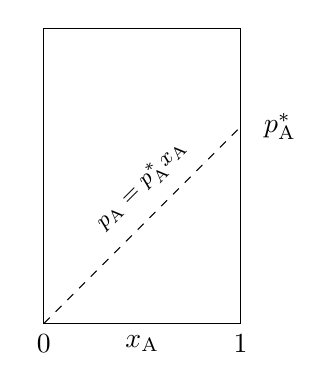
\begin{tikzpicture}[scale=2.5]
                \draw[] (0,0) rectangle (1,1.5);
                \draw[dashed] (0,0)--(1,1);
                \node at (0,-0.1) {0};
                \node at (0.5,-0.1) {$x_\mathrm{A}$};
                \node at (1,-0.1) {1};
                \node at (1.2,1) {$p_\mathrm{A}^*$};
                \node [rotate =45] at (0.5,0.7) {\footnotesize $p_\mathrm{A}=p_\mathrm{A}^*x_\mathrm{A}$};
            \end{tikzpicture}
        \end{center}
    \end{minipage}

    在定温定压下，任一组分在全部浓度范围内都符合拉乌尔定律的溶液，称为\highlight{理想溶液}。
\end{frame}


\begin{frame}[t]
    \begin{example}
        308K时，丙酮的饱和蒸气压为$\SI{4.3e4}{Pa}$，今测得$x_{\text{氯仿}}=0.3$的氯仿-丙酮溶液蒸气中丙酮蒸气的分压为$\SI{2.7e4}{Pa}$，问此溶液是否为理想溶液？
    \end{example}
\end{frame}


\begin{frame}[t]
    \frametitle{}
    \begin{example}
        由A和B组成近似的理想溶液，在B的摩尔分数为0.03，温度为370.26K时，溶液的蒸气压为$\SI{101325}{Pa}$，已知纯A在该温度下的饱和蒸气压是$\SI{91293.8}{Pa}$。计算相同温度时，B的摩尔分数为0.02的溶液上方
        
        （1）A的蒸气分压；（2）B的蒸气分压。
    \end{example}
    \pause
    \[
        \begin{aligned}
            p_\mathrm{A}&=p_\mathrm{A}^* x_\mathrm{A} = 91293.8\times (1-0.02) = 89467.9 \,\mathrm{Pa} \\
            p &= p_\mathrm{A}^* x_\mathrm{A} + p_\mathrm{B}^* x_\mathrm{B} \\
            101325 &= 91293.8\times (1-0.03) + p_\mathrm{B}^* \times 0.03 \\
            p_\mathrm{B}^* &= 425667 \,\mathrm{Pa} \\
            p_\mathrm{B}&=p_\mathrm{B}^* x_\mathrm{B} = 425667 \times 0.02 = 8513.34 \,\mathrm{Pa}
        \end{aligned}
    \]
\end{frame}



\begin{frame}{理想溶液中各组分的化学势}
    由两种或两种以上易挥发物质组成的理想溶液，在定温定压条件下，溶液的蒸气相与液相达到平衡时，根据相平衡条件，溶液中任一组分B在液相和气相中的化学势相等，即$\mu_\mathrm{B}(l)=\mu_\mathrm{B}(g)$。若将蒸气看作理想气体，则
    $$\mu_\mathrm{B}(l)=\mu_\mathrm{B}(g)=\mu_{\mathrm{B}}^\ominus(T) +R T \ln \frac{p_{\mathrm{B}}}{p^{\ominus}}$$
    根据拉乌尔定律，将$p_\mathrm{B}=p_\mathrm{B}^*x_\mathrm{B}$代入，并去掉气、液标记 
    \[
        \begin{aligned}
            \mu_\mathrm{B}&=\mu_{\mathrm{B}}^\ominus(T) +R T \ln \frac{p_{\mathrm{B}}^*}{p^{\ominus}}+RT\ln x_\mathrm{B} \\
            &= \mu_{\mathrm{B}}^*(T,p_\mathrm{B}^*) +R T \ln x_\mathrm{B}
        \end{aligned}
    \]
\end{frame}


\begin{frame}{理想溶液中各组分的化学势}
    \[
        \mu_\mathrm{B}= \mu_{\mathrm{B}}^*(T,p_\mathrm{B}^*) +R T \ln x_\mathrm{B}
    \]
    当$x_\mathrm{B}=1$时，$\mu_{\mathrm{B}}^*(T,p_\mathrm{B}^*)$是纯组分B的化学势，它是温度和压力的函数。选取温度$T$和压力$p$($p$为溶液上面混合蒸气各组分平衡分压之和)时，纯液体状态作为理想溶液中组分B的标准态。而压力$p$对$\mu_{\mathrm{B}}^*$的影响不大，所以$\mu_{\mathrm{B}}^*(T,p_\mathrm{B}^*) \approx \mu_{\mathrm{B}}^*(T,p)$。这样上式可写成
    \maincolor{$$\mu_\mathrm{B}=\mu_{\mathrm{B}}^*(T,p)+R T \ln x_\mathrm{B}$$}
    上式为理想溶液中任一组分B的化学势公式，也是理想溶液的热力学定义式。任一组分的化学势均可用上式表示的溶液即为理想溶液。
\end{frame}


\begin{frame}[t]{}
    \begin{example}
        （1）同种理想气体分别处于298K、110kPa及310K、110kPa，写出气体两种状态的化学势表达式，并判断两种状态的化学势$\mu$和标准化学势$\mu^\ominus$是否相等；
        \\（2）写出同温同压下纯苯和苯-甲苯理想溶液中组分苯的化学势，并判断苯的两种状态的$\mu^*$、$\mu$是否相等。
    \end{example}
\end{frame}


\begin{frame}{亨利定律}
    亨利(Henry)总结了挥发性溶质在稀溶液的溶解度与其平衡分压的关系时指出：定温下，稀溶液中挥发性溶质的平衡分压$(p_\mathrm{B})$与其在溶液中的浓度$x_\mathrm{B}$成正比。
    $$p_\mathrm{B}=k_x x_\mathrm{B}$$
    式中$k_x$为亨利常量，它与溶质、溶剂的性质及温度、压力和浓度的表示方法等有关。溶质的浓度还可用物质的量浓度$c_\mathrm{B}$、质量摩尔浓度$b_\mathrm{B}$表示，$T$、$p$一定时
    $$p_\mathrm{B}=k_x x_\mathrm{B}=k_c c_\mathrm{B}=k_b b_\mathrm{B}$$
    由于溶质浓度表示方法不同，亨利常量各不相同，$k_x\neq k_c \neq k_b$。
    
    亨利定律适用于{\color{red}稀溶液}，而且要求溶质在气、液两相中具有相同的分子状态。
    
    \highlight{理想稀溶液}：定温定压下，在一定浓度范围内，溶剂服从拉乌尔定律，溶质服从亨利定律的稀溶液称为理想稀溶液(或稀溶液)。
\end{frame}


\begin{frame}{稀溶液中溶剂的化学势}
    定温定压下，在一定浓度范围内，溶剂服从拉乌尔定律，溶质服从亨利定律的稀溶液称为理想稀溶液(或稀溶液)。
    \\由于稀溶液中溶剂A遵守拉乌尔定律，因此稀溶液中溶剂的化学势表示式应与理想溶液中各组分化学势表示式相同，溶剂A的化学势为
    $$\mu_\mathrm{A}=\mu_{\mathrm{A}}^*(T,p)+R T \ln x_\mathrm{A}$$
    式中$\mu_{\mathrm{A}}^*(T,p)$为$x_\mathrm{A}=1$时纯溶剂的化学势。即稀溶液中溶剂的标准态就是$T$、$p$条件下的纯溶剂。
\end{frame}



\begin{frame}{稀溶液中溶质的化学势}
    在一定$T$、$p$下，稀溶液中溶质B在气液两相达平衡时，
    $$\mu_\mathrm{B}(l)=\mu_\mathrm{B}(g)=\mu_{\mathrm{B}}^\ominus(T) +R T \ln \frac{p_{\mathrm{B}}}{p^{\ominus}}$$
    因稀溶液中溶质服从亨利定律，将$p_\mathrm{B}=k_x x_\mathrm{B}$代入得
    $$\mu_\mathrm{B}(l)=\mu_\mathrm{B}(g)=\mu_{\mathrm{B}}^\ominus(T) +R T \ln \frac{k_x}{p^{\ominus}}+RT \ln x_\mathrm{B}=\mu_{\mathrm{B},x}^\ominus(T,p)+RT\ln x_\mathrm{B}$$
    式中，$\mu_{\mathrm{B},x}^\ominus(T,p)$为溶质B摩尔分数$x_\mathrm{B}=1$在标准态时的标准化学势。这个标准态对B是不存在的，因为当$x_\mathrm{B}=1$时，溶液已不是理想稀溶液，这个状态是假想的状态。
\end{frame}


\begin{frame}{稀溶液中溶质的化学势}
    \begin{columns}[c]
        \column{6.75cm}
            
\includegraphics[width=6cm]{figs/fig2.2.png}
        \column{6.75cm}
            如图所示，图中$k_\mathrm{B}$点是理想稀溶液中溶质B的标准态，它不同于实际存在的纯溶质状态$p_\mathrm{B}^*$点，$\mu_{\mathrm{B},x}^\ominus(T,p)$是假想的$k_\mathrm{B}$点的化学势，而不是状态$p_\mathrm{B}^*$点的化学势$\mu_{\mathrm{B}}^*(T,p)$，即$\mu_{\mathrm{B},x}^\ominus(T,p) \neq \mu_{\mathrm{B}}^*(T,p)$。
    \end{columns}
\end{frame}


\begin{frame}{稀溶液中溶质的化学势}
实际应用中，溶质的浓度还可以用物质的量浓度$c$、质量摩尔浓度$b$表示，由于$p_\mathrm{B}=k_{\mathrm{B},c}c_\mathrm{B}$，$p_\mathrm{B}=k_{\mathrm{B},b}b_\mathrm{B}$，还可以得到
\begin{table}
        \begin{tabular}{l l}        
        $\mu_{\mathrm{B}}=\mu_{\mathrm{B},x}^\ominus(T,p)+RT\ln x_\mathrm{B}$ & $\qquad\mu_{\mathrm{B},x}^\ominus(T,p)=\mu_{\mathrm{B}}^\ominus(T) +R T \ln \frac{k_x}{p^{\ominus}}$ \\        
        \specialrule{0em}{3pt}{3pt} 
        $\mu_{\mathrm{B}}=\mu_{\mathrm{B}, c}^{\ominus}(T, p)+R T \ln \frac{c_{\mathrm{B}}}{c^{\ominus}}$ & $\qquad \mu_{\mathrm{B}, c}^{\ominus}(T, p)=\mu_{\mathrm{B}}^{\ominus}(T)+R T \ln \frac{k_{\mathrm{B}, c} c_{\mathrm{B}}^{\ominus}}{p^{\ominus}}$ \\
        \specialrule{0em}{3pt}{3pt} 
        $\mu_{\mathrm{B}}=\mu_{\mathrm{B}, b}^{\ominus}(T, p)+R T \ln \frac{b_{\mathrm{B}}}{b^{\ominus}}$ & $\qquad \mu_{\mathrm{B}, b}^{\ominus}(T, p)=\mu_{\mathrm{B}}^{\ominus}(T)+R T \ln \frac{k_{\mathrm{B}, b} b_{\mathrm{B}}^{\ominus}}{p^{\ominus}}$ \\
        \end{tabular}
\end{table}
    虽然都表示稀溶液中溶质B的化学势，但由于浓度的表示方法不同，它们的标准态化学势也互不相同，即$\mu_{\mathrm{B}, x}^{\ominus}(T, p) \neq \mu_{\mathrm{B}, c}^{\ominus}(T, p) \neq \mu_{\mathrm{B}, b}^{\ominus}(T, p)$，但溶质的化学势$\mu_\mathrm{B}$无论用何种浓度表示都是一样的。
\end{frame}


\begin{frame}{理想溶液的通性 $\Delta_\mathrm{mix}V=0$}
    定温定组成下，将式$\mu_\mathrm{B}=\mu_{\mathrm{B}}^*(T,p_\mathrm{B}^*)+R T \ln x_\mathrm{B}$对$p$求偏微商
    $$\left(\frac{\partial \mu_{\mathrm{B}}}{\partial p}\right)_{T, n}=\left\{\frac{\partial}{\partial p}\left[\mu_{\mathrm{B}}^{*}(T, p)+R T \ln x_{\mathrm{B}}\right]\right\}_{T, n}=\left[\frac{\partial \mu_{\mathrm{B}}^{*}(T, p)}{\partial p}\right]_{T, n}$$
    得
    $$V_\mathrm{B,m}=V_\mathrm{m}(\mathrm{B})$$
    即理想溶液中任一组分的偏摩尔体积等于纯物质的摩尔体积。又因为
    $$\Delta_\mathrm{mix}V=\sum_Bn_\mathrm{B}V_{\mathrm{B,m}}-\sum_Bn_\mathrm{B}V_\mathrm{m}(\mathrm{B})=0$$
    所以在理想溶液形成的过程中无体积的变化。
\end{frame}


\begin{frame}{理想溶液的通性 $\Delta_\mathrm{mix}S>0$}
    定压定组成条件下，将式$\mu_\mathrm{B}=\mu_{\mathrm{B}}^*(T,p_\mathrm{B}^*)+R T \ln x_\mathrm{B}$对$T$求偏微商
    $$\left(\frac{\partial \mu_{\mathrm{B}}}{\partial T}\right)_{p, n}=\left\{\frac{\partial}{\partial T}\left[\mu_{\mathrm{B}}^{*}(T, p)+R T \ln x_{\mathrm{B}}\right]\right\}_{p, x}=\left[\frac{\partial \mu_{\mathrm{B}}^{*}(T, p)}{\partial T}\right]_{P, n}+R\ln x_\mathrm{B}$$
    得
    $$S_\mathrm{B,m}=S_\mathrm{m}(\mathrm{B})-R\ln x_\mathrm{B}$$
    而$$\Delta_{\text {mix }} S=\sum_{\mathrm{B}} n_{\mathrm{B}} S_{\mathrm{B}, \mathrm{m}}-\sum_{\mathrm{B}} n_{\mathrm{B}} S_{\mathrm{m}}(\mathrm{B})=-\sum_{\mathrm{B}} R n_{\mathrm{B}} \ln x_{\mathrm{B}}>0$$
    所以由纯组分混合形成理想溶液的混合过程熵增大。
\end{frame}


\begin{frame}{理想溶液的通性 $\Delta_\mathrm{mix}G<0$}
    设混合前和混合后体系的吉布斯自由能分别为$G_1$和$G_2$，则
    $$G_{1}=\sum_{\mathrm{B}} n_{\mathrm{B}} G_{\mathrm{m}}(\mathrm{B})=\sum_{\mathrm{B}} n_{\mathrm{B}} \mu_{\mathrm{B}}^{*}(T, p)$$
    $$G_{2}=\sum_{\mathrm{B}} n_{\mathrm{B}} G_{\mathrm{B}, \mathrm{m}}=\sum_{\mathrm{B}} n_{\mathrm{B}} \mu_{\mathrm{B}}^{*}(T, p)+R T \sum_{\mathrm{B}} n_{\mathrm{B}} \ln x_{\mathrm{B}}$$
    混合过程
    $$\Delta_{\text {mix }} G=G_{2}-G_{1}=R T \sum_{\mathrm{B}} n_{\mathrm{B}} \ln x_{\mathrm{B}}<0$$
    所以由纯组分混合形成理想溶液的混合过程吉布斯自由能减小。
\end{frame}


\begin{frame}{理想溶液的通性 $\Delta_\mathrm{mix}H=0$}
    定温下，
    $$\Delta G=\Delta H - T\Delta S$$
    所以
    $$\Delta_{\mathrm{mix}} H=\Delta_{\mathrm{mix}} G + T\Delta_{\mathrm{mix}} S = 0$$
\end{frame}


\begin{frame}{非理想溶液中各组分的化学势}
    非理想溶液（nonideal solution）中由于各组分分子间作用力不同，或溶剂浓度不是很大、溶质浓度不是很小，造成溶剂不服从拉乌尔定律，溶质不服从亨利定律，这样的溶液既不是理想溶液，也不是理想稀溶液。为了使非理想稀溶液中物质的化学势公式也具有简单的形式，路易斯提出活度（activity）的概念，用活度a代替浓度。令
    $$a=\gamma x$$
    式中：$a$称为相对活度，简称活度；$\gamma$为活度系数(activity coefficient)；$a$与$\gamma$均为量纲1的数。
    $\gamma$与溶质、溶剂性质有关，还与溶液的浓度、温度有关。
\end{frame}


\begin{frame}{非理想溶液中溶剂的化学势}
    引入活度概念后，拉乌尔定律为
    $$p_{\mathrm{A}}=p_{\mathrm{A}}^{*} a_{\mathrm{A}, x} \qquad a_{\mathrm{A}, x}=\gamma_{\mathrm{A}, x} x_{\mathrm{A}}$$
    引入活度概念后，亨利定律为\\
    $$\begin{aligned}
        p_{\mathrm{B}}=k_{x} a_{\mathrm{B}, x} & a_{\mathrm{B}, x}=\gamma_{\mathrm{B}, x} x_{\mathrm{B}} \\
        p_{\mathrm{B}}=k_{c} a_{\mathrm{B}, c} & a_{\mathrm{B}, c}=\gamma_{\mathrm{B}, c} c_{\mathrm{B}} / c^{\ominus} \\
        p_{\mathrm{B}}=k_{\mathrm{b}} a_{\mathrm{B}, \mathrm{b}} & a_{\mathrm{B}, \mathrm{b}}=\gamma_{\mathrm{B}, \mathrm{b}} b_{\mathrm{B}} / b^{\ominus}
        \end{aligned}$$
    非理想溶液中溶剂的化学势为
    $$\mu_{\mathrm{A}}=\mu_{\mathrm{A}}^{*}(T, p)+R T \ln a_{\mathrm{A}}$$
\end{frame}


\begin{frame}{非理想溶液中溶质的化学势}
    用活度表示的溶剂的化学势为
    $$\left\{\begin{array}{l}
        \mu_{\mathrm{B}}=\mu_{\mathrm{B}, x}^{\ominus}(T, p)+R T \ln a_{\mathrm{B}, x} \\
        \mu_{\mathrm{B}}=\mu_{\mathrm{B}, c}^{\ominus}(T, p)+R T \ln a_{\mathrm{B}, c} \\
        \mu_{\mathrm{B}}=\mu_{\mathrm{B}, \mathrm{b}}^{\ominus}(T, p)+R T \ln a_{\mathrm{B}, \mathrm{b}}
        \end{array}\right.$$
    式中：$\mu_{\mathrm{B}, x}^{\ominus}(T, p)$为温度$T$、标准压力$p^\ominus$下，$a_{\mathrm{B}, x}=1, \gamma_{\mathrm{B}, x}=1, x_{\mathrm{B}}=1$时仍能服从亨利定律的溶质的假想态；
    \\$\mu_{\mathrm{B}, c}^{\ominus}(T, p)$为温度$T$、标准压力$p^\ominus$下，$a_{\mathrm{B}, c}=1, \gamma_{\mathrm{B}, c}=1, c_{\mathrm{B}}=1 \si{mol.dm^{-3}}$时仍能服从亨利定律的溶质的假想态；
    \\$\mu_{\mathrm{B}, b}^{\ominus}(T, p)$为$T$、$p^\ominus$下，$a_{\mathrm{B}, b}=1, \gamma_{\mathrm{B}, b}=1, b_{\mathrm{B}}=1 \si{mol.kg^{-3}}$时溶质的假想态。
\end{frame}